\documentclass{standalone}
\usepackage{tikz}
\usepackage{bm}
\usetikzlibrary{decorations.pathmorphing, patterns, arrows, decorations.markings}
\begin{document}

\pgfarrowsdeclarecombine{dimarrow}{dimarrow}{latex}{latex}{}{}
    \def\Dimline[#1][#2][#3][#4]{
        \path #1 -- node (#4) {\emph{$#4$}} #3;
        \draw[-|,
        decoration={markings, 
                mark=at position 1 with {};,
            },
        postaction=decorate] (#4) -- #1;
        \draw[|-,
        decoration={markings, 
                mark=at position 0 with {};,
            },
        postaction=decorate] #3 -- (#4);
    }

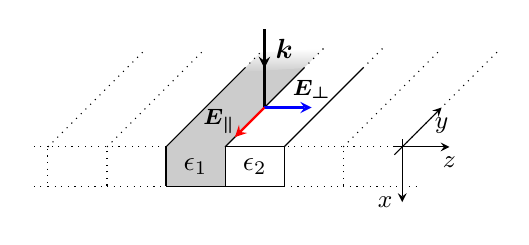
\begin{tikzpicture}
    
    % Center two blocks
    \draw[fill=gray!40] (0,0) -- (0.75,0) -- (0.75,0.5) -- (0,0.5) -- (0,0);
    \draw (0.75,0) -- (1.5,0) -- (1.5,0.5) -- (0.75,0.5);
    
    % backline
    %\draw (0,0.5) -- (0.75,1.25) -- (1.5,1.25) -- (0.75,0.5);
    
    \draw[fill=gray!40, draw=none] (0,0.5) -- (1,1.5) -- (1.75,1.5) -- (0.75,0.5) -- (0,0.5);
    \shade[bottom color=gray!40, top color=white] (1.2,1.7) -- (2.0,1.75) -- (1.75,1.5) -- (0.95,1.45) -- (1.25,1.75);
    \draw (0,0.5) -- (1,1.5);
    \draw[dotted] (1,1.5) -- (1.25,1.75);
    
    \draw (0.75,0.5) -- (1.75,1.5);
    \draw[dotted] (1.75,1.5) -- (2.0,1.75);
    
    % backline
    %\draw (1.5,0.5) -- (2.25,1.25) -- (1.5,1.25);
    \draw (1.5,0.5) -- (2.5,1.5);
    \draw[dotted] (2.5,1.5) -- (2.75,1.75);
    
    % behind
    %\draw (1.5,0) -- (2.25,0.75) -- (2.25,1.25);
    
    % Ghost blocks(ters), left
    \draw[dotted] (-1.5,0) -- (-0.75,0) -- (-0.75,0.5) -- (-1.5,0.5) -- (-1.5,0);
    \draw[dotted] (-0.75,0) -- (0,0);
    \draw[dotted] (0,0.5) -- (-0.75,0.5);
    
    % backline 
    %\draw[dotted] (-1.5,0.5) -- (-0.75,1.25) -- (0,1.25);
    \draw[dotted] (-1.5,0.5) -- (-0.25,1.75);
    
    %backline 
    %\draw[dotted] (-0.75,0.5) -- (0,1.25) -- (0.75,1.25);
    \draw[dotted] (-0.75,0.5) -- (0.5,1.75);
    
    % behind
    %\draw[dotted] (-1.5,0) -- (-0.75,0.75) -- (-0.75,1.25);
    %\draw[dotted] (-0.75,0) -- (0,0.75) -- (0,1.25);
    %\draw[dotted] (-0.75,0.75) -- (0.2,0.75);
    
    % Ghost blocks(ters), right
    \draw[dotted] (1.5,0) -- (2.25,0) -- (2.25,0.5) -- (1.5,0.5);
    \draw[dotted] (2.25,0) -- (3,0) -- (3,0.5) -- (2.25,0.5);
    
    % backline
    %\draw[dotted] (3,0.5) -- (3.75,1.25) -- (1.75,1.25);
    \draw[dotted] (3,0.5) -- (4.25,1.75);
    
    % behind
    %\draw[dotted] (3,0) -- (3.75,0.75) -- (3.75,1.25);
    
    \draw[dotted] (2.25,0.5) -- (3.5,1.75);
    
    % small continuation indication lines
    \draw[dotted] (-1.5,0)--(-1.75,0);
    \draw[dotted] (-1.5,0.5)--(-1.75,0.5);
    %\draw[dotted] (-0.75,1.25)--(-1,1.25);
    \draw[dotted] (3,0)--(3.25,0);
    \draw[dotted] (3,0.5)--(3.25,0.5);
    
    % behind
    %\draw[dotted] (2.25,0.75) -- (3.75,0.75);
    %\draw[dotted] (2.25,0) -- (3,0.75) -- (3,1.25);
    
    % dimlines
    \Dimline[(0,-0.25)][(0.375,-0.25)][(0.75,-0.25)][a];
    \Dimline[(0.74,-0.25)][(1.125,-0.25)][(1.5,-0.25)][b];
    
    \node at (0.375,0.25) {$\epsilon_1$};
    \node at (1.125,0.25) {$\epsilon_2$};
    
    % k arrow
    \draw[thick] (1.25,1) -- (1.25,2);
    \draw[thick, <-, >=stealth] (1.25,1.5) -- (1.25,2);
    \draw[thick, blue, ->, >=stealth] (1.25,1) -- (1.85,1);
    \draw[thick, red, ->, >=stealth] (1.25,1) -- (0.875,0.625);
    
    % coordinate system axes
    \draw[->, >=stealth] (2.9,0.5) -- (3.6,0.5) node[below] {\small $z$};
    \draw[->, >=stealth] (3,0.6) -- (3,-0.2) node[left] {\small $x$};
    \draw[->, >=stealth] (2.9,0.4) -- (3.5,1) node[below] {\small $y$};
    
    % labels
    \node at (1.5,1.75) {$\bm{k}$};
    \node at (1.85,1.23) {\footnotesize $\bm{E_{\bot}}$};
    \node at (0.675,0.825) {\footnotesize $\bm{E_{\parallel}}$};
    
    
    
\end{tikzpicture}
\end{document}